% Section content template for individual Educative lessons
% This file contains the actual content for a specific section
% Generated from Educative API section content

% Section: Activity Diagram for the Car Rental System
% Section ID: 6111367285440512
% Section Slug: activity-diagram-for-the-car-rental-system
% Generated: 2025-12-12T14:51:54.952804

Activity diagrams are a great way to visualize the flow of messages from one activity to another in the system. There can be different activity diagrams that we can create for our car rental system. In this lesson, we will create activity diagrams for the following two activities:

\begin{itemize}
\item
\protect\phantomsection\label{BeFE21S9WKHbo359Ffo6L}
Vehicle pickup
\item
\protect\phantomsection\label{DxWsvVD1rw8-iuBakrQCi}
\textbf{Activity challenge:} Vehicle return
\end{itemize}

\subsection{Vehicle pickup}\label{33y-VE1Cyghis4IlFKTOD}
\\
The states and actions involved in this activity diagram are given below.

\subsubsection{States}\label{RNBCdY5FFIjCJTQtnVvTO}
\\
\textbf{Initial state:} A member with a vehicle booking comes to the ``rent a car'' reception to pick up the vehicle.
\\
\textbf{Final state:} The guest successfully gets the vehicle, or the system shows a reservation error.

\subsubsection{Actions}\label{PtA_QyUFnFsIrLiTIA1M0}
\\
When a member with a vehicle reservation arrives at the rent-a-car reception, the receptionist validates the reservation and updates the vehicle status.
\\
Based on the order above, the activity diagram of the vehicle pickup from the car rental facility is given below.

\begin{figure}[htbp]
 \centering
 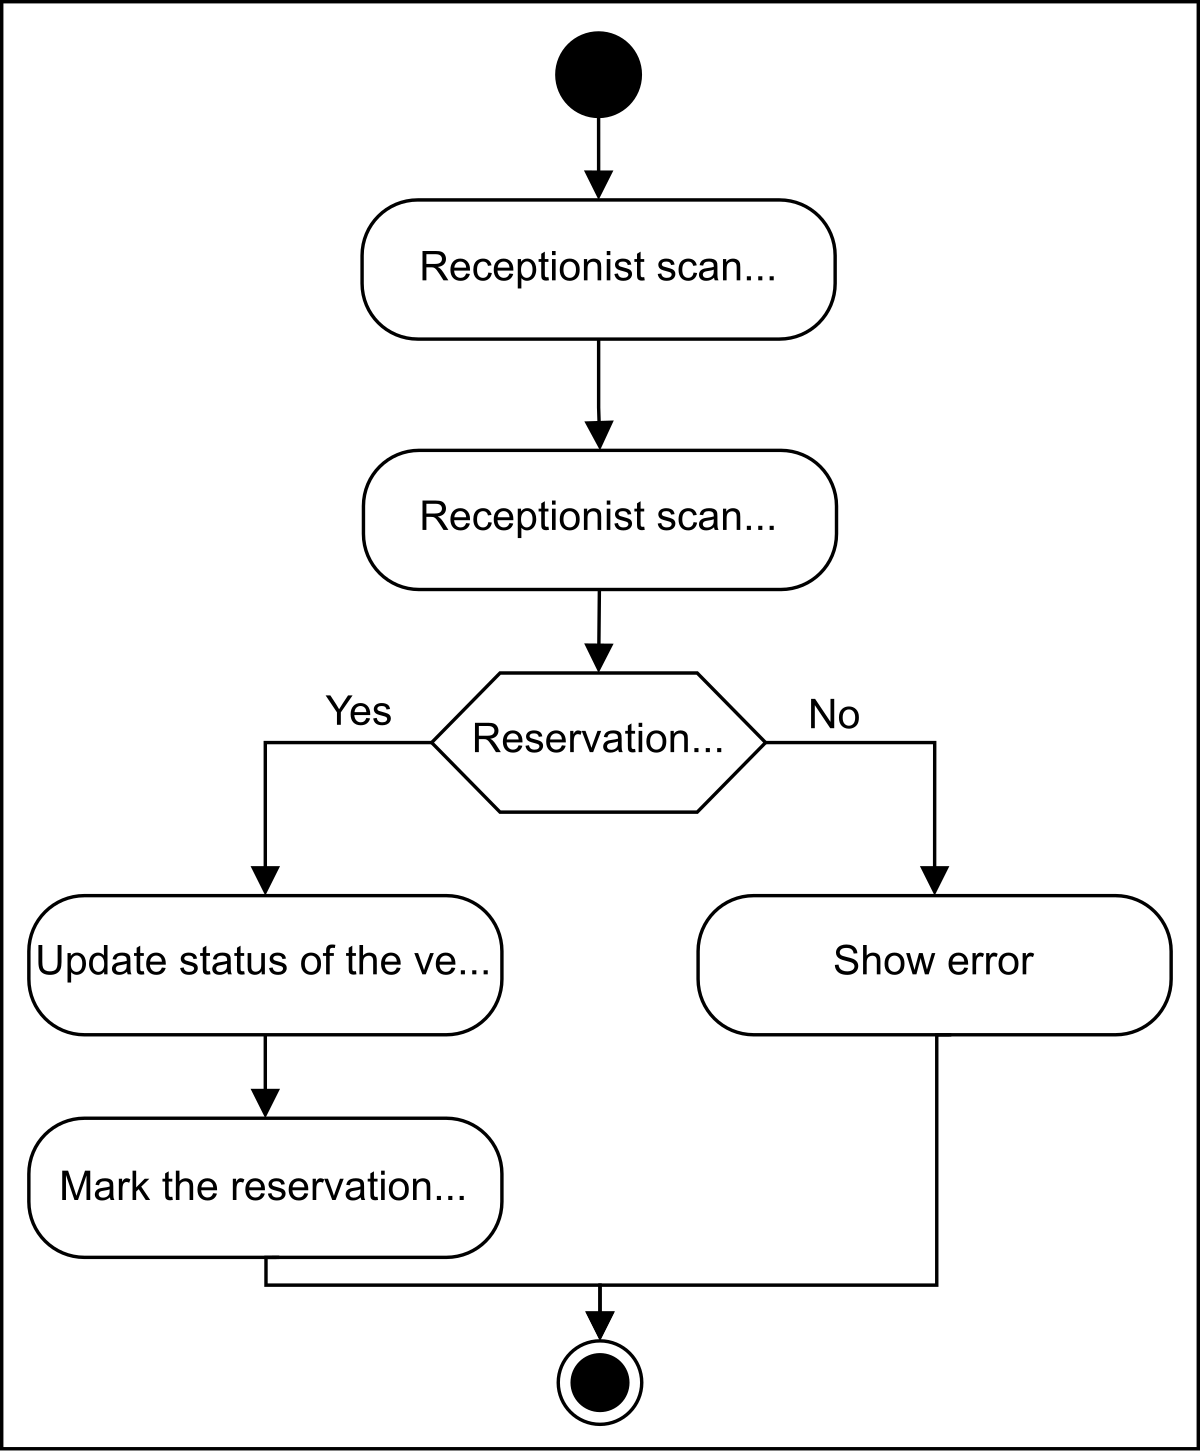
\includegraphics[width=0.5\textwidth]{Images/chapter_15/section_6111367285440512/4809828347412480.png}
 \caption{The activity diagram for vehicle pickup}
\end{figure}

\subsection{Activity challenge: Vehicle return}\label{qQ8UiLDWEEf6Cnibbq9TJ-2}
\\
You will help us create an activity diagram of a member who wants to return the vehicle.
\\
Here is the activity diagram structure:

\begin{figure}[htbp]
 \centering
 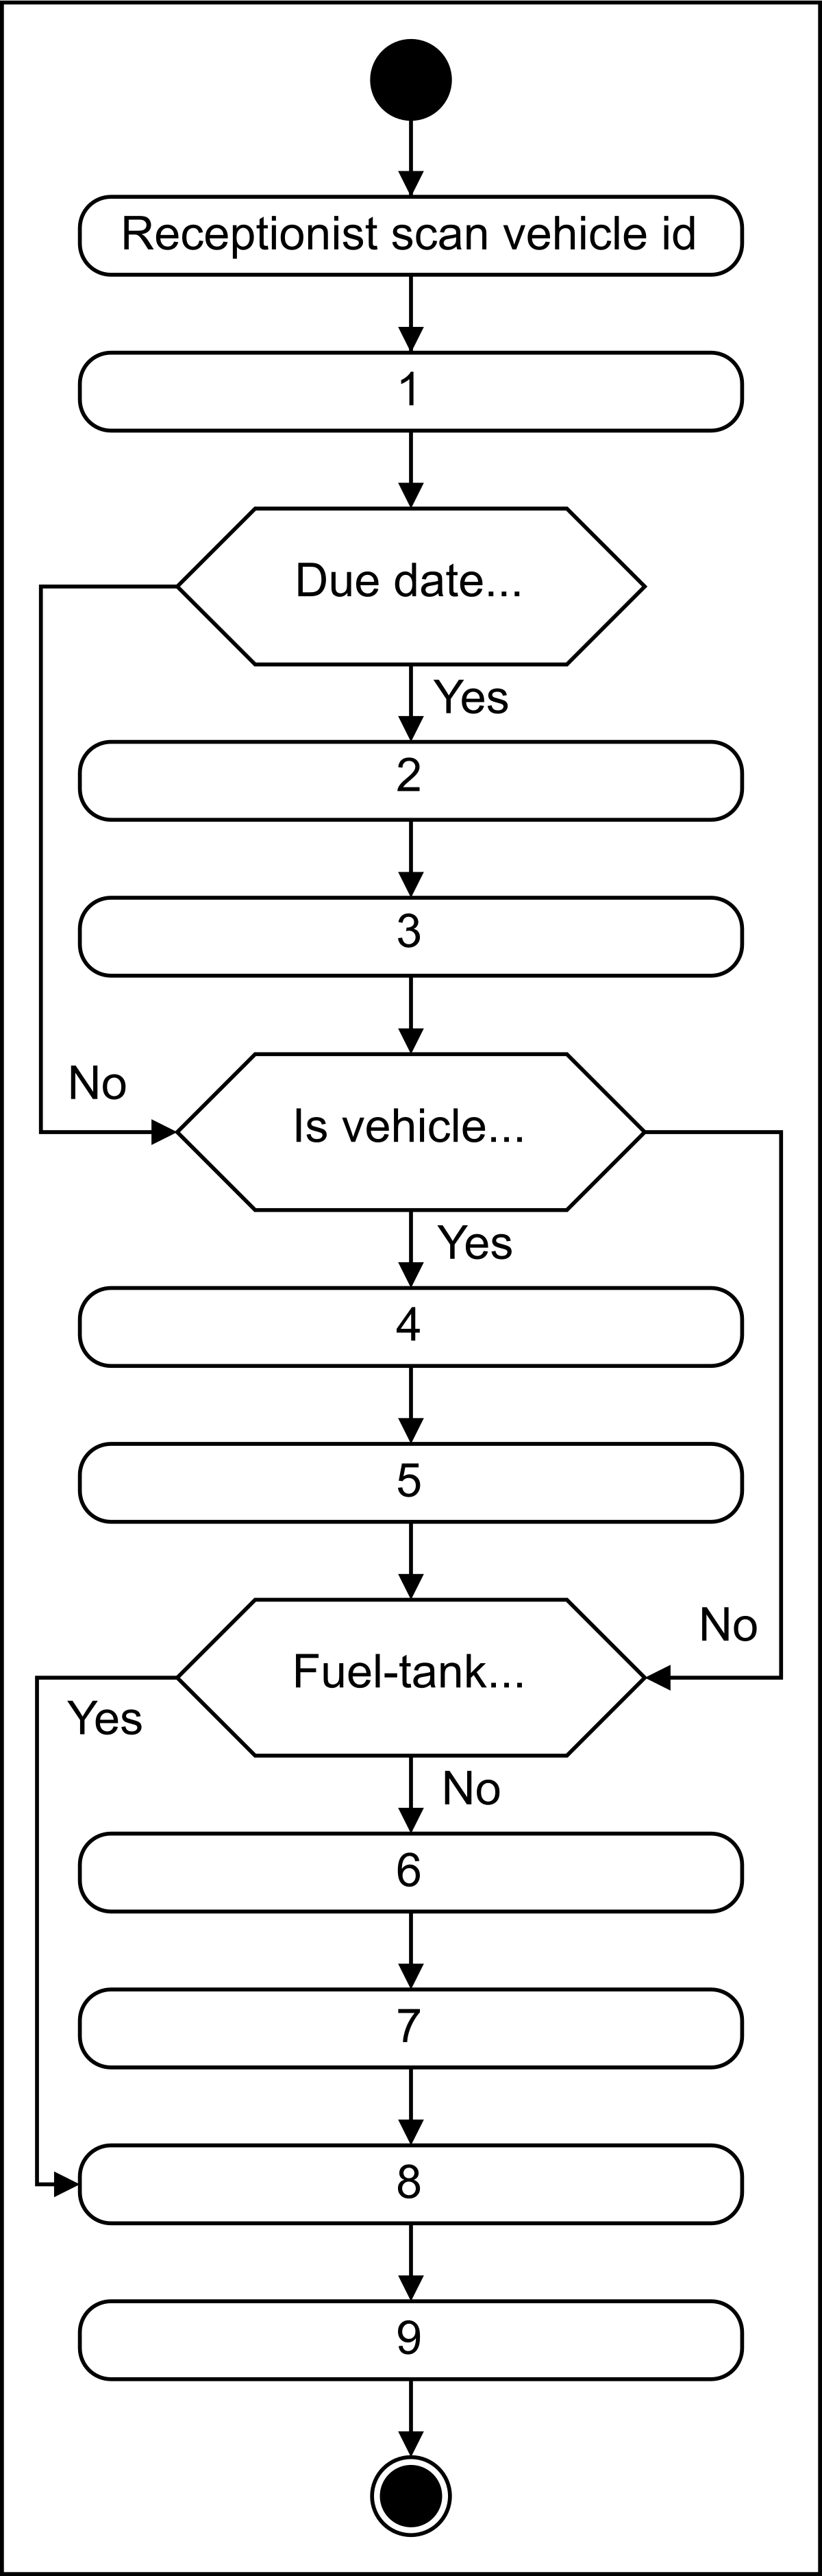
\includegraphics[width=0.5\textwidth]{Images/chapter_15/section_6111367285440512/4973584223305728.png}
 \caption{The activity diagram for vehicle return}
\end{figure}

Notice that the actions in the diagram above are numbered from 1 to 9. The slots below represent the activities, and the arrows represent the flow from one activity to another. Can you rearrange the slots below in the correct order they should appear in the activity diagram above?
\begin{quote}
\textbf{Note:} If you're stuck, click the ``Show Solution'' button.
\end{quote}

Alternatively, you can also click the ``Show complete diagram'' button below to view the complete sequence diagram of the cancel reservation interaction.

We've looked at some of our car rental system's activity diagrams. In the next lesson, we will present the code for our designed classes in some of the most popular languages.

% End of section content